\documentclass[12pt]{article}
\usepackage{graphicx}
\usepackage{amsmath}
\usepackage{amssymb}
\usepackage{amsthm}


\makeindex
\begin{document}

\title{Proyecto de Modelos Matemáticos Aplicados }
\author{Ana Karla Caballero Gonzales C411 \\ Alejandro Camacho Pérez C412}

\date{}

\maketitle



\section{Introduction}
En una investigación anterior realizada en la facultad de Matemática y Computación de la Universidad de La Habana, MATCOM, se proponía basándose en trabajos anteriores varios modelos matemáticos para modelar y resolver problemáticas relacionadas con el acto sexual. En el mismo se plantean los siguientes 5 problemas:

\begin{enumerate}
    \item Maximizar la duración del acto sexual.
    \item Maximizar el placer del que menor placer alcance al finalizar el acto sexual.
    \item Minimizar el cansancio del participante con mayor cansancio al finalizar el acto sexual.
    \item Minimizar la energía inicial de todos los participantes de forma que al terminar todos hayan alcanzado el orgasmo y tengan la misma energía.
    \item Maximizar el placer inicial de un participante específico, de forma tal que todos los participantes, excepto el específico, alcancen el orgasmo.
\end{enumerate}

El objetivo de este trabajo, es hacer una implementación, utilizando un lenguaje de programación, de los modelos matemáticos propuestos en dicha investigación.

\section{Cuestiones Generales de los problemas}

La investigación realizada utilizó los siguientes parámetros:

\subsection{Datos}
\begin{itemize}
    \item $J = \{1 \dots j\}$: Conjunto de participantes.
    \item $N = \{1 \dots n\}$: Posturas a adoptar
    \item $A_{ij}$: Energía de la persona $j$ al terminar la postura $i\  \forall i = \overline{1,n}$.
    \item $P_{ij}$: Placer de la persona $j$ al terminar la postura $i$. $i\  \forall i = \overline{1,n}$. y $i\  \forall j \in J$.
    \item $\widehat{p}_j$: Placer necesario para que la persona $j$ alcance el orgasmo. $\forall j \in J$.
    \item $T_i$: Tiempo empleado en la postura $i$. $\forall i = \overline{1,n}$.
    \item $C_{ij}$ : Cantidad de energía que consume la postura $i$ al participante j por unidad de tiempo $\forall i = \overline{1,n}$ y $\forall j \in J$.
    \item $Pa_{ij}$:Cantidad de placer que otorga la postura $i$ al participante $j$ por unidad de tiempo. $\forall i = \overline{1,n}$ y $\forall j \in J$
    
\end{itemize}

\subsection{Variables}
\begin{itemize}
    \item $X_i$: Tiempo empleado en la postura $i$. $\forall i = \overline{1,n}$.
    \item $Pp_{ok}$: Placer inicial del participante $k$, $k\in J$. (Sólo el problema 5)
    \item  $E_{0j}$: Energía inicial de la persona $j$. $\forall j \in J$. (Sólo el problema 4)
\end{itemize}

\subsection{Restricciones comunes}

\begin{itemize}
    \item Después de cada postura, la energía disminuye de manera proporcional al tiempo que se permanezca en ella: $$ A_{ij} = A_{(i-i)j}-C_{ij}X_{i} \ \forall i \in N \ \forall j \in J$$
    \item Después de cada postura, el placer de cada participante aumenta de manera proporcional al tiempo que se permanezca en ella: $$ P_{ij}=P_{(i-1)j}+P_{ij}X_{i} \ \forall i \in N \ \forall j \in J $$
    \item En todo momento la energía es mayor igual que cero $$ A_{ij}\geq 0 \ \forall i \in N \ \forall j \in J  $$
    \item El placer después del acto sexual es mayor o igual al placer necesario para alcanzar el orgasmo $$ P_{nj}\geq \widehat{P}_j \ \forall j \in J $$
\end{itemize}

\section{Sobre la implementación}

La implementación del trabajo fue hecha en Python, utilizando la librería pulp para la resolución de problemas de programación lineal. El mismo consta de dos módulos principales, uno para la interfaz de usuario y la comunicación del mismo con el programa, y otro para la resolución de los problemas.

\subsection{Módulo de interfaz de usuario}

La interfaz de usuario ofrece la posibilidad de:

\begin{itemize}
    \item Crea, editar y eliminar participantes.
    \item Crea, editar y eliminar posturas.
    \item Listar participantes y posturas con todos sus detalles.
    \item Exportar e importar los datos de los participantes y posturas a un archivo de json.
    \item Seleccionar y resolver uno de los problemas planteados.
\end{itemize}


\newpage
\begin{figure}
    \centering
    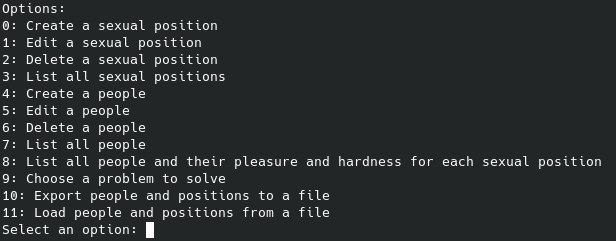
\includegraphics[width=0.7\textwidth]{images/ui_example.png}
    \caption{Interfaz de usuario}
    \label{fig:interfaz}
\end{figure}

\subsubsection{Uso de la interfaz de usuario}

La interfaz de usuario sigue las siguientes constantes:

\begin{itemize}
    \item Para la creación de una nueva postura es necesario sólo indicar su nombre
    \item Para la creación de un nuevo participante es necesario indicar su nombre, placer necesario para alcanzar el orgasmo y energía inicial. Así cómo también los valores de energía y placer para cada postura.
    \item Tras modificar un participante, se pedirá actualizar los valores de energía y placer para cada postura.
    \item Tras añadir una postura si existían participantes, se pedirá actualizar los valores de energía y placer para cada participante.
    \item La letra c cancela la acción que se esté realizando por completo.
\end{itemize}

Tras tener al menos un participante y una postura, se puede seleccionar uno de los problemas planteados y resolverlo. El programa entonces pasa a enviar los datos en un formato adecuado al módulo de resolución de problemas.

\subsection{Módulo de resolución de problemas}

El módulo de resolución de problemas consta de una clase abstracta, AbstractProblem, que encapsula el procedimiento para cada problema, utilizando los métodos objetive\_function, constraints y solve. Cada problema hereda de esta clase abstracta y sobrescribe los métodos mencionados. Para poder resolver un problema, es necesaria la creación de una clase que herede de AbstractProblem y sobrescriba los métodos mencionados.

% TODO: Introducir foto del código
\begin{figure}
    \centering
    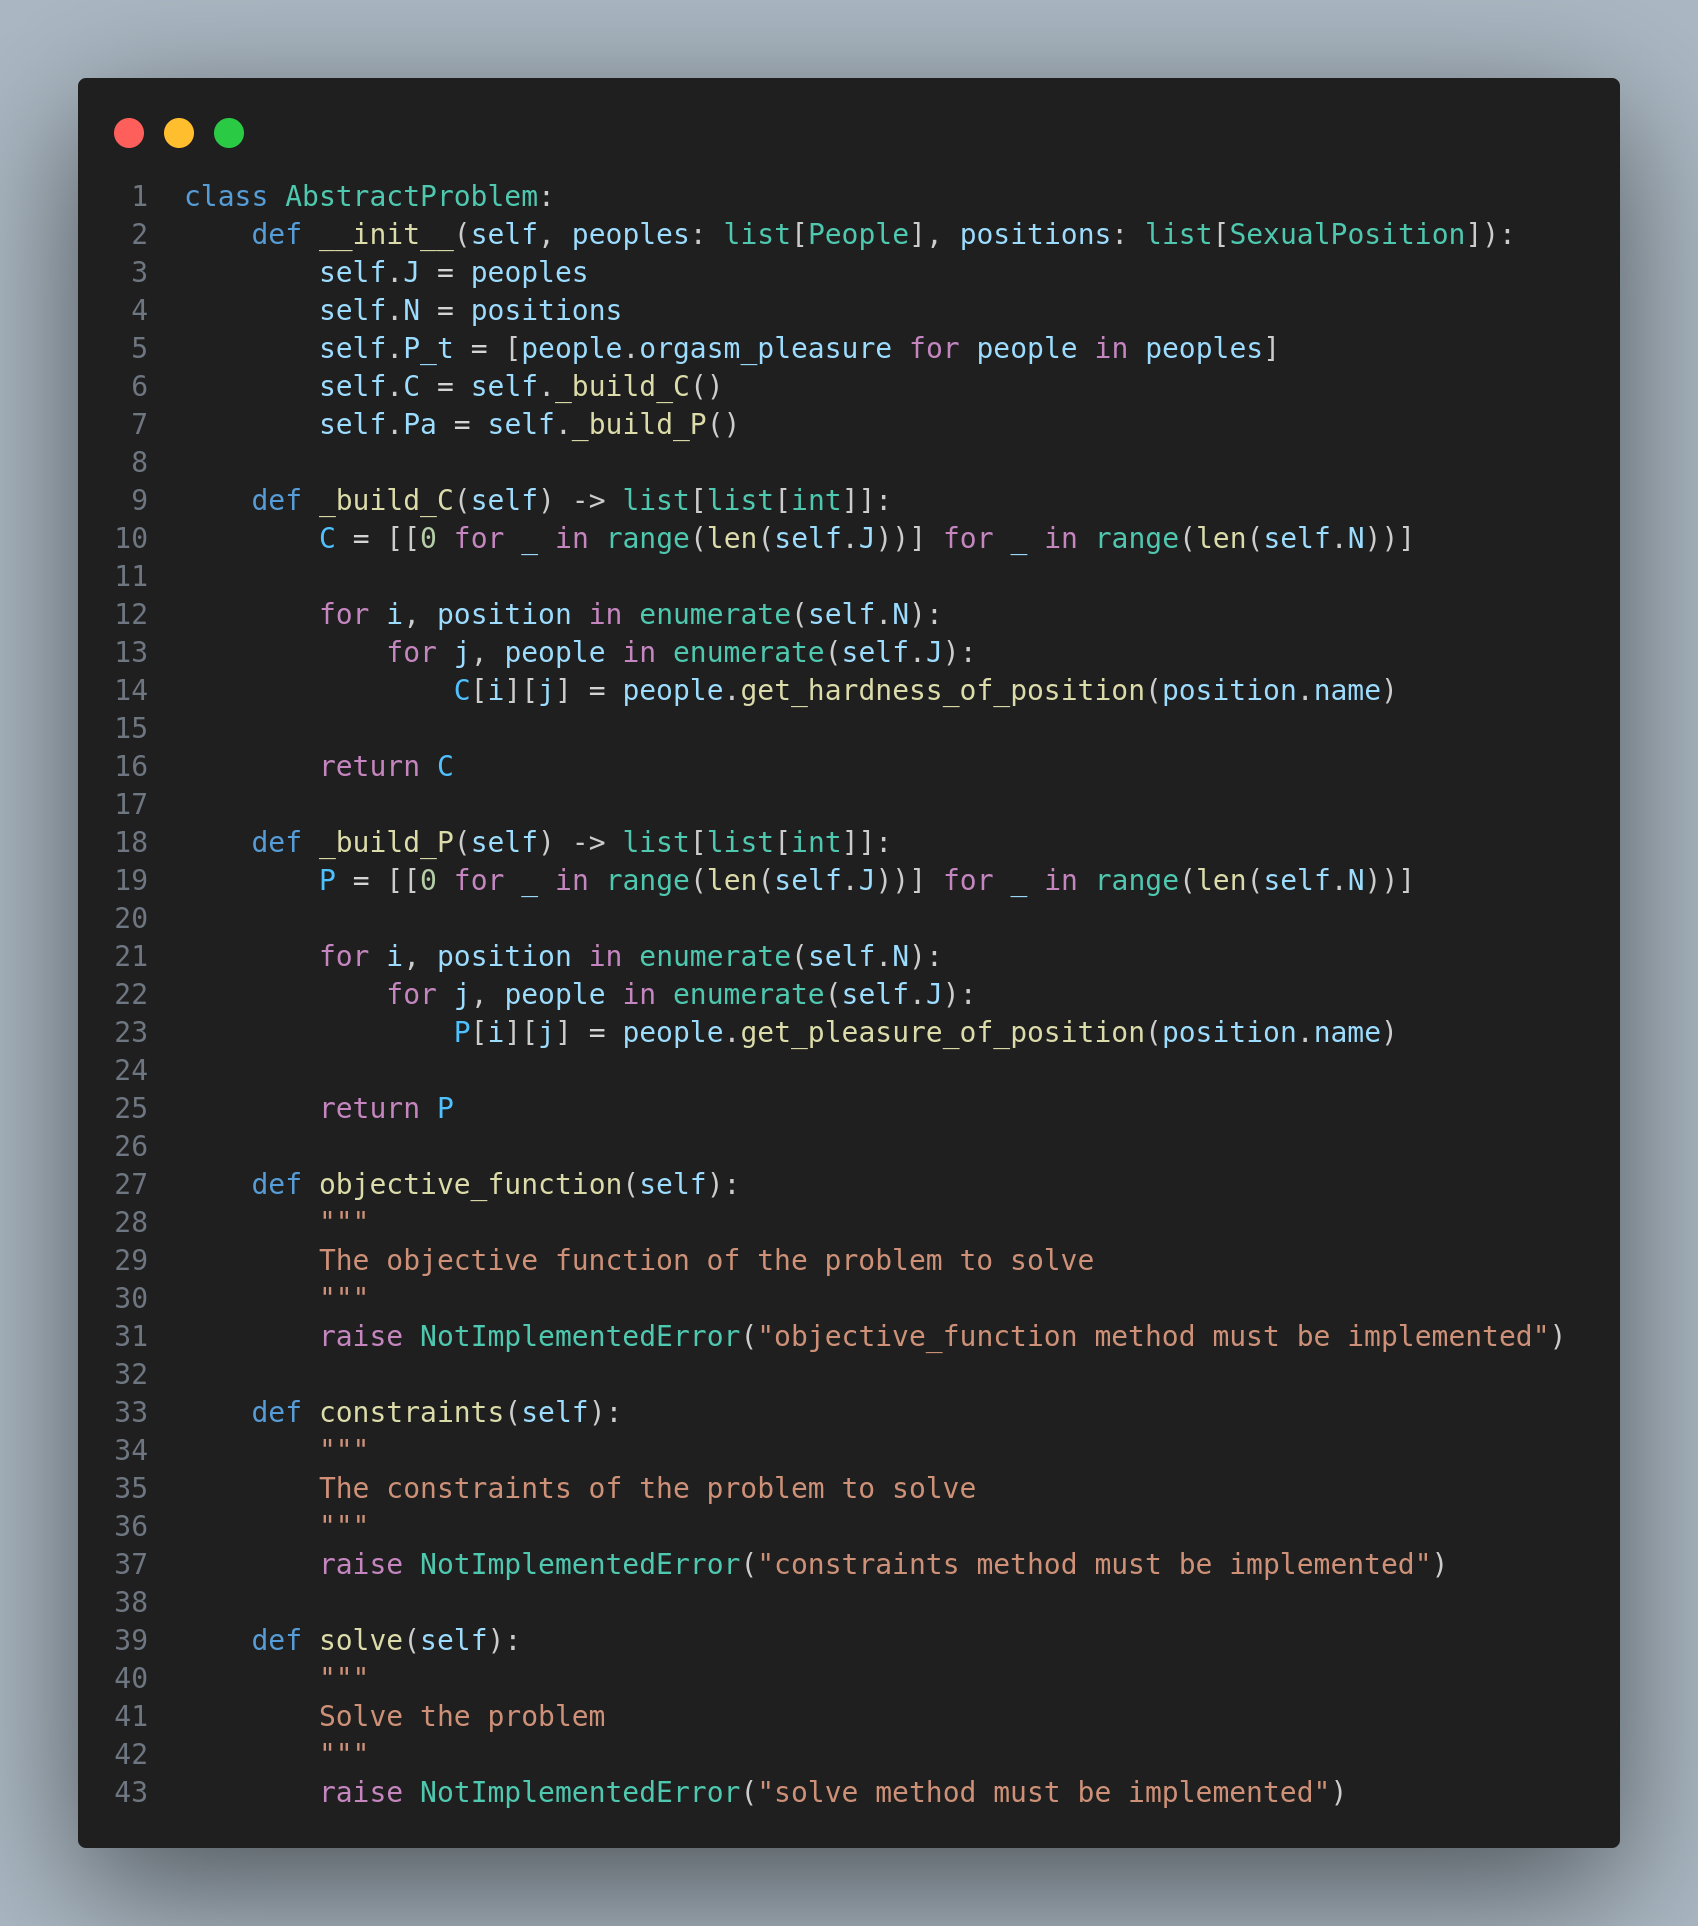
\includegraphics[width=0.7\textwidth]{images/abstract.png}
    \caption{Clase AbstractProblem}
    \label{fig:abstract}
\end{figure}

\begin{figure}
    \centering
    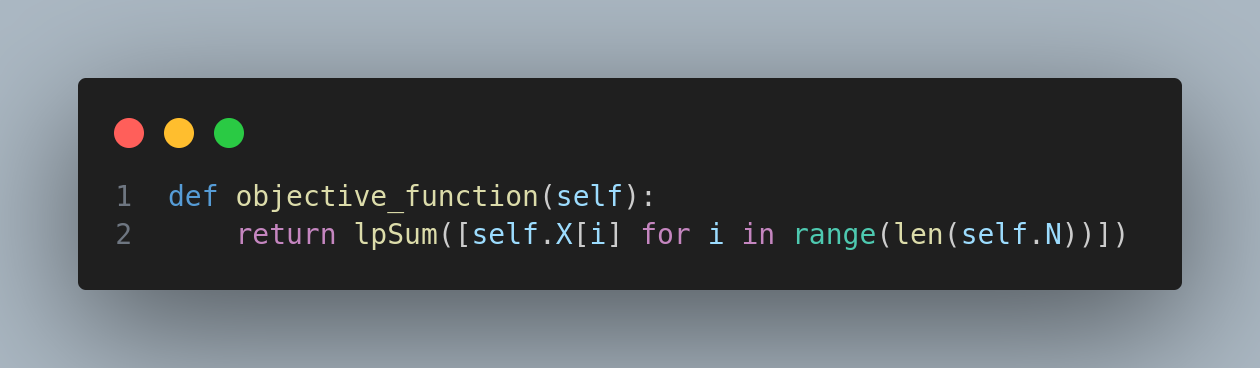
\includegraphics[width=0.7\textwidth]{images/max_objetive.png}
    \caption{Función objetivo para el problema 1}
    \label{fig:fop1}
\end{figure}

\begin{figure}
    \centering
    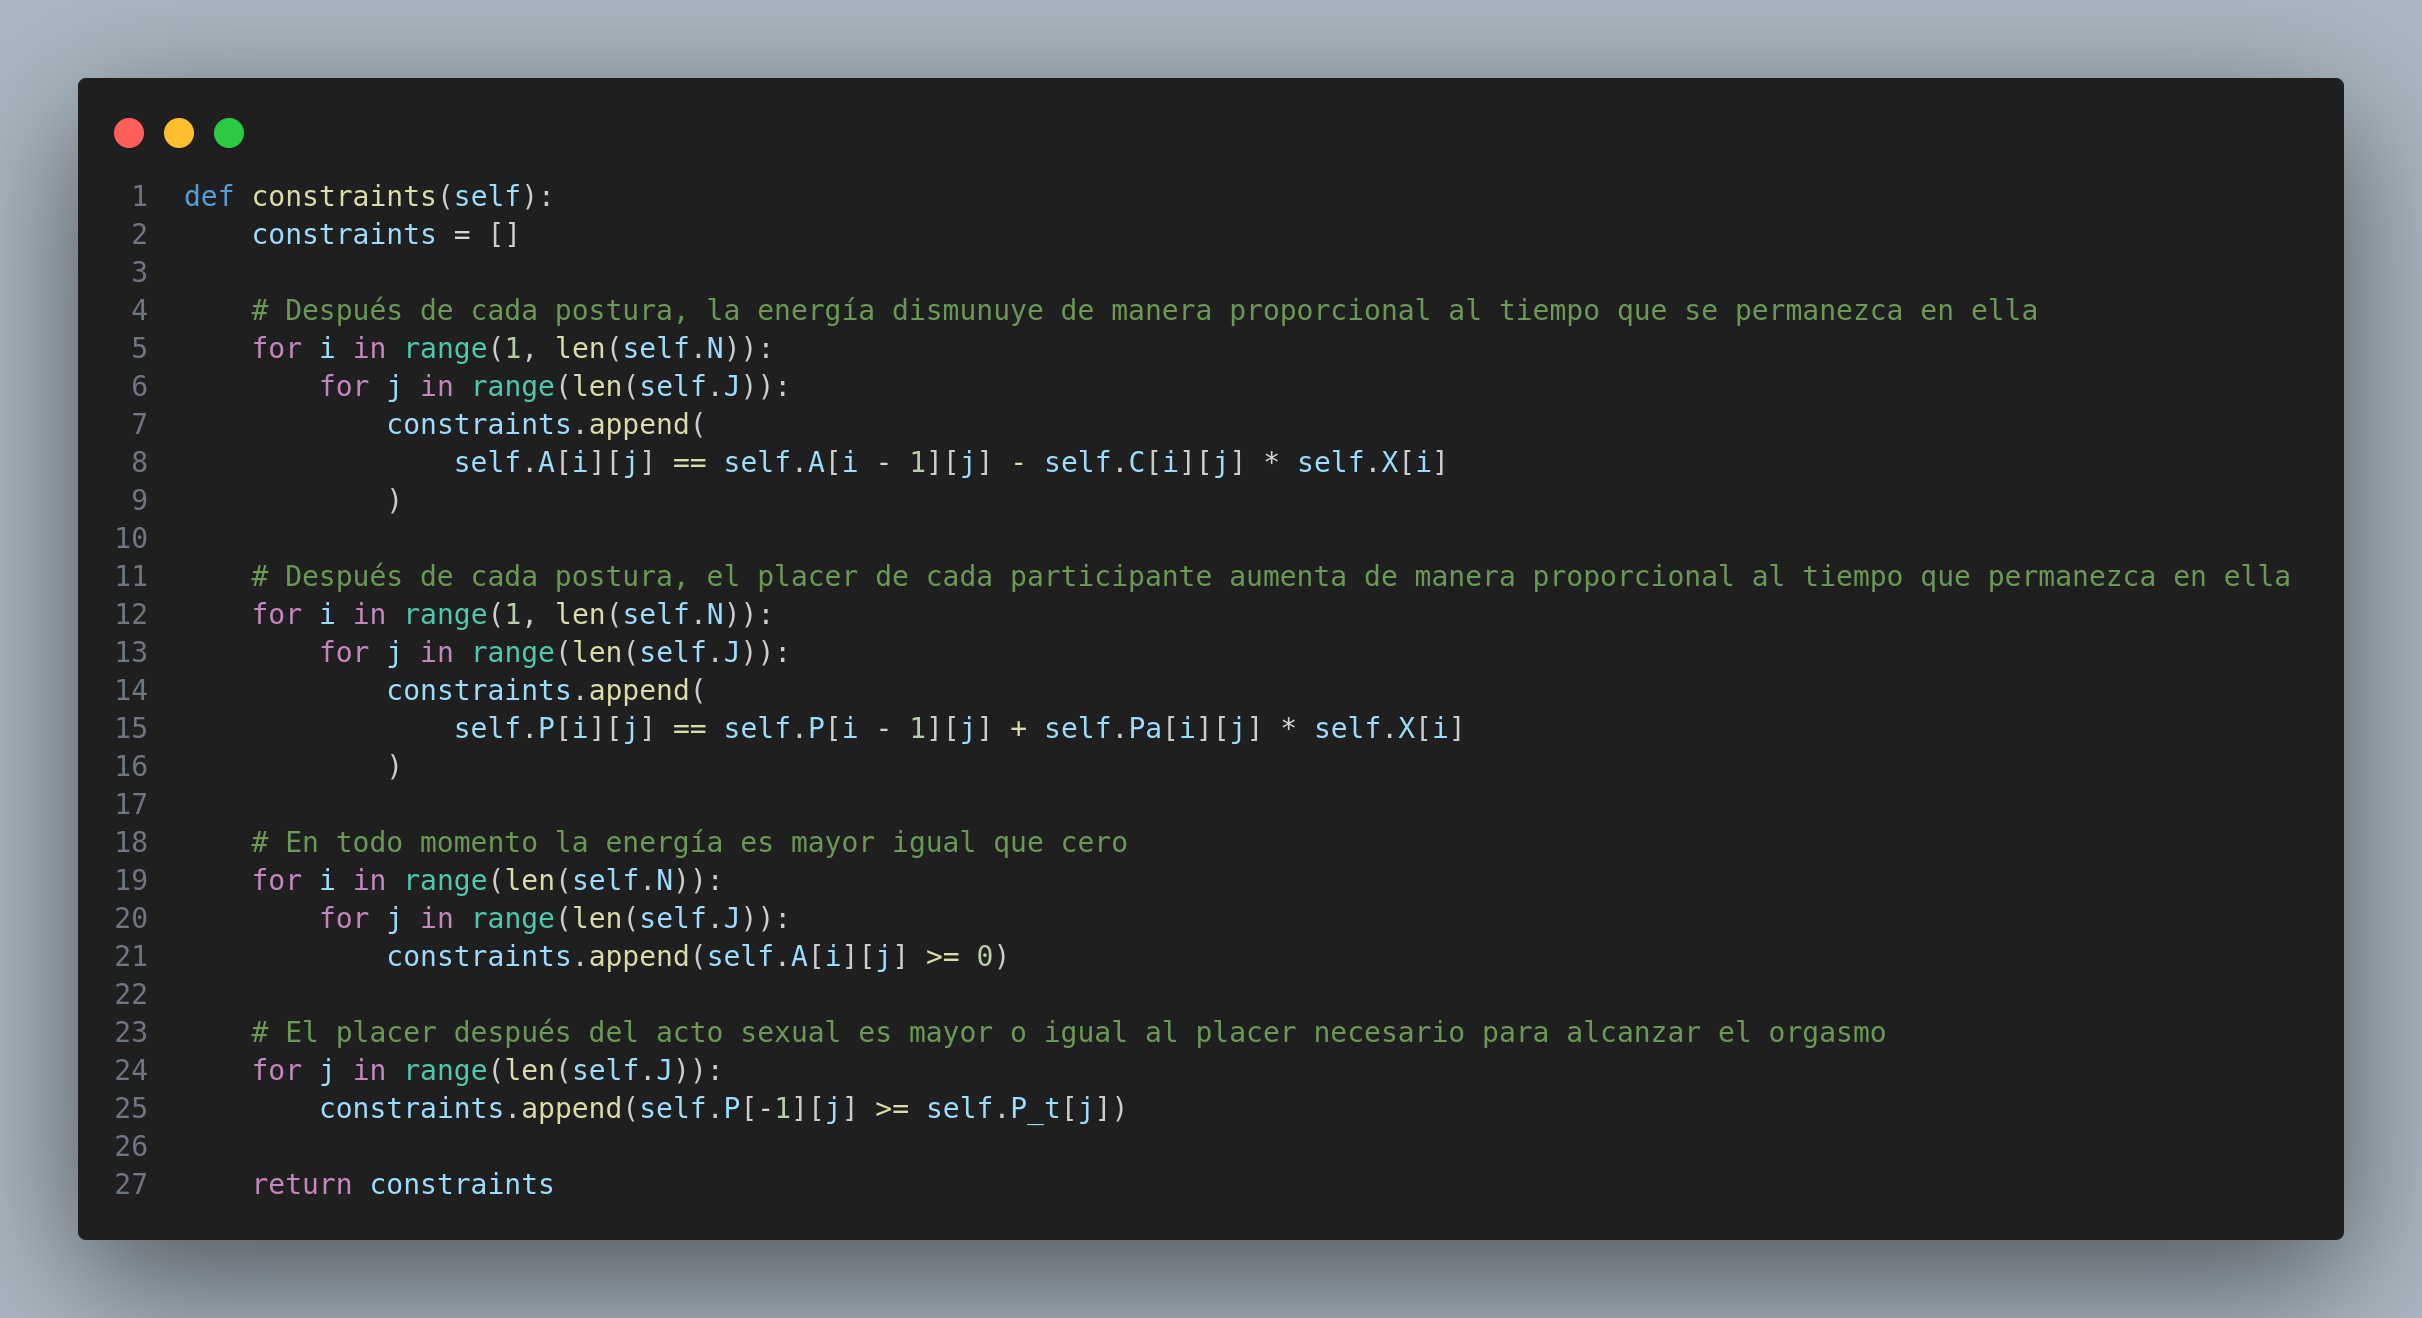
\includegraphics[width=0.7\textwidth]{images/max_constraints.png}
    \caption{Restricciones para el problema 1}
    \label{fig:rp1}
\end{figure}

\begin{figure}
    \centering
    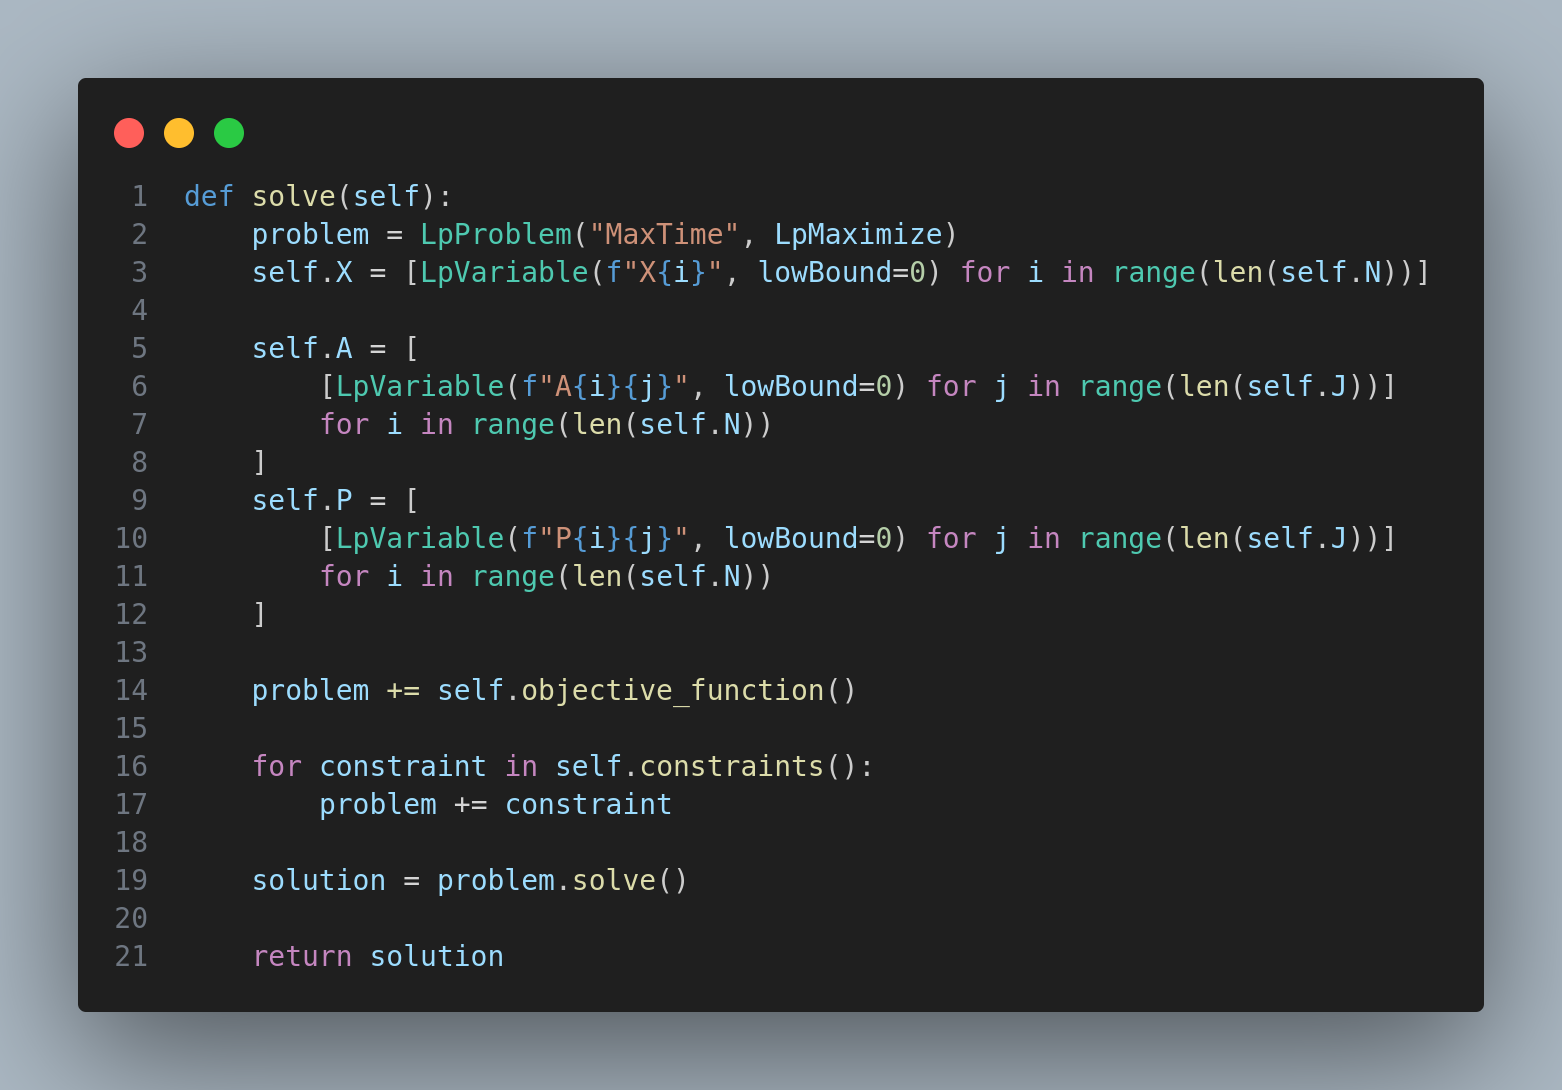
\includegraphics[width=0.7\textwidth]{images/max_solve.png}
    \caption{Resolución del problema 1}
    \label{fig:rs1}
\end{figure}

\begin{figure}
    \centering
    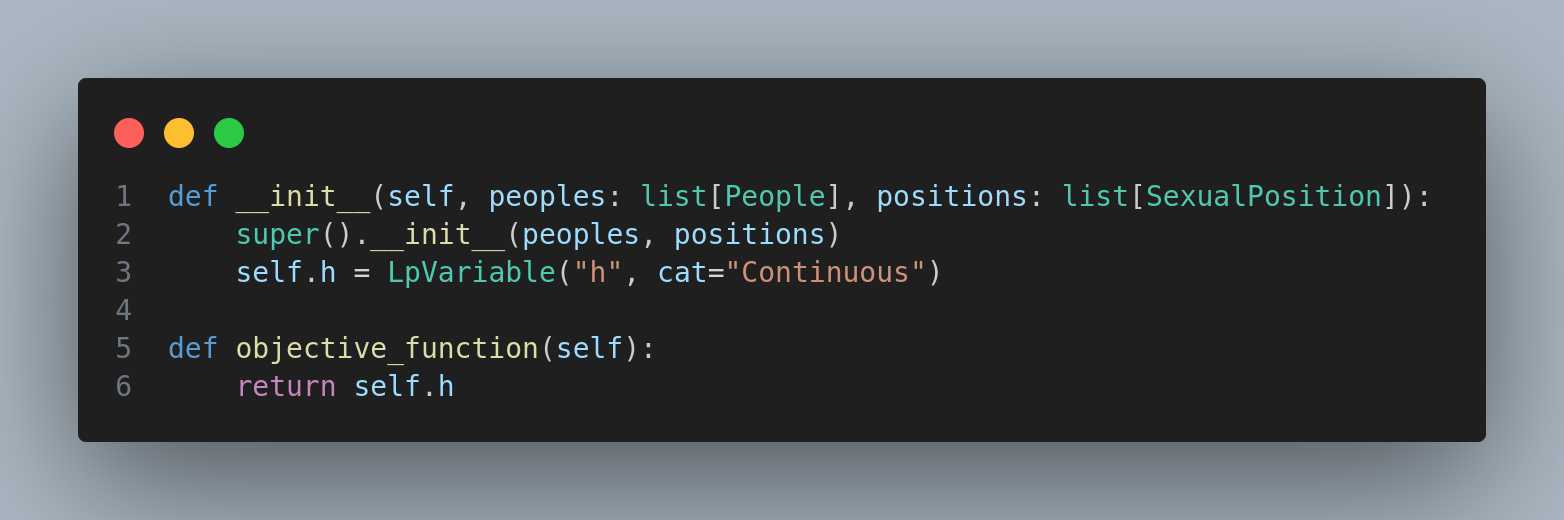
\includegraphics[width=0.7\textwidth]{images/max_min_objetive.png}
    \caption{Función objetivo para el problema 2}
    \label{fig:fop2}
\end{figure}

\begin{figure}
    \centering
    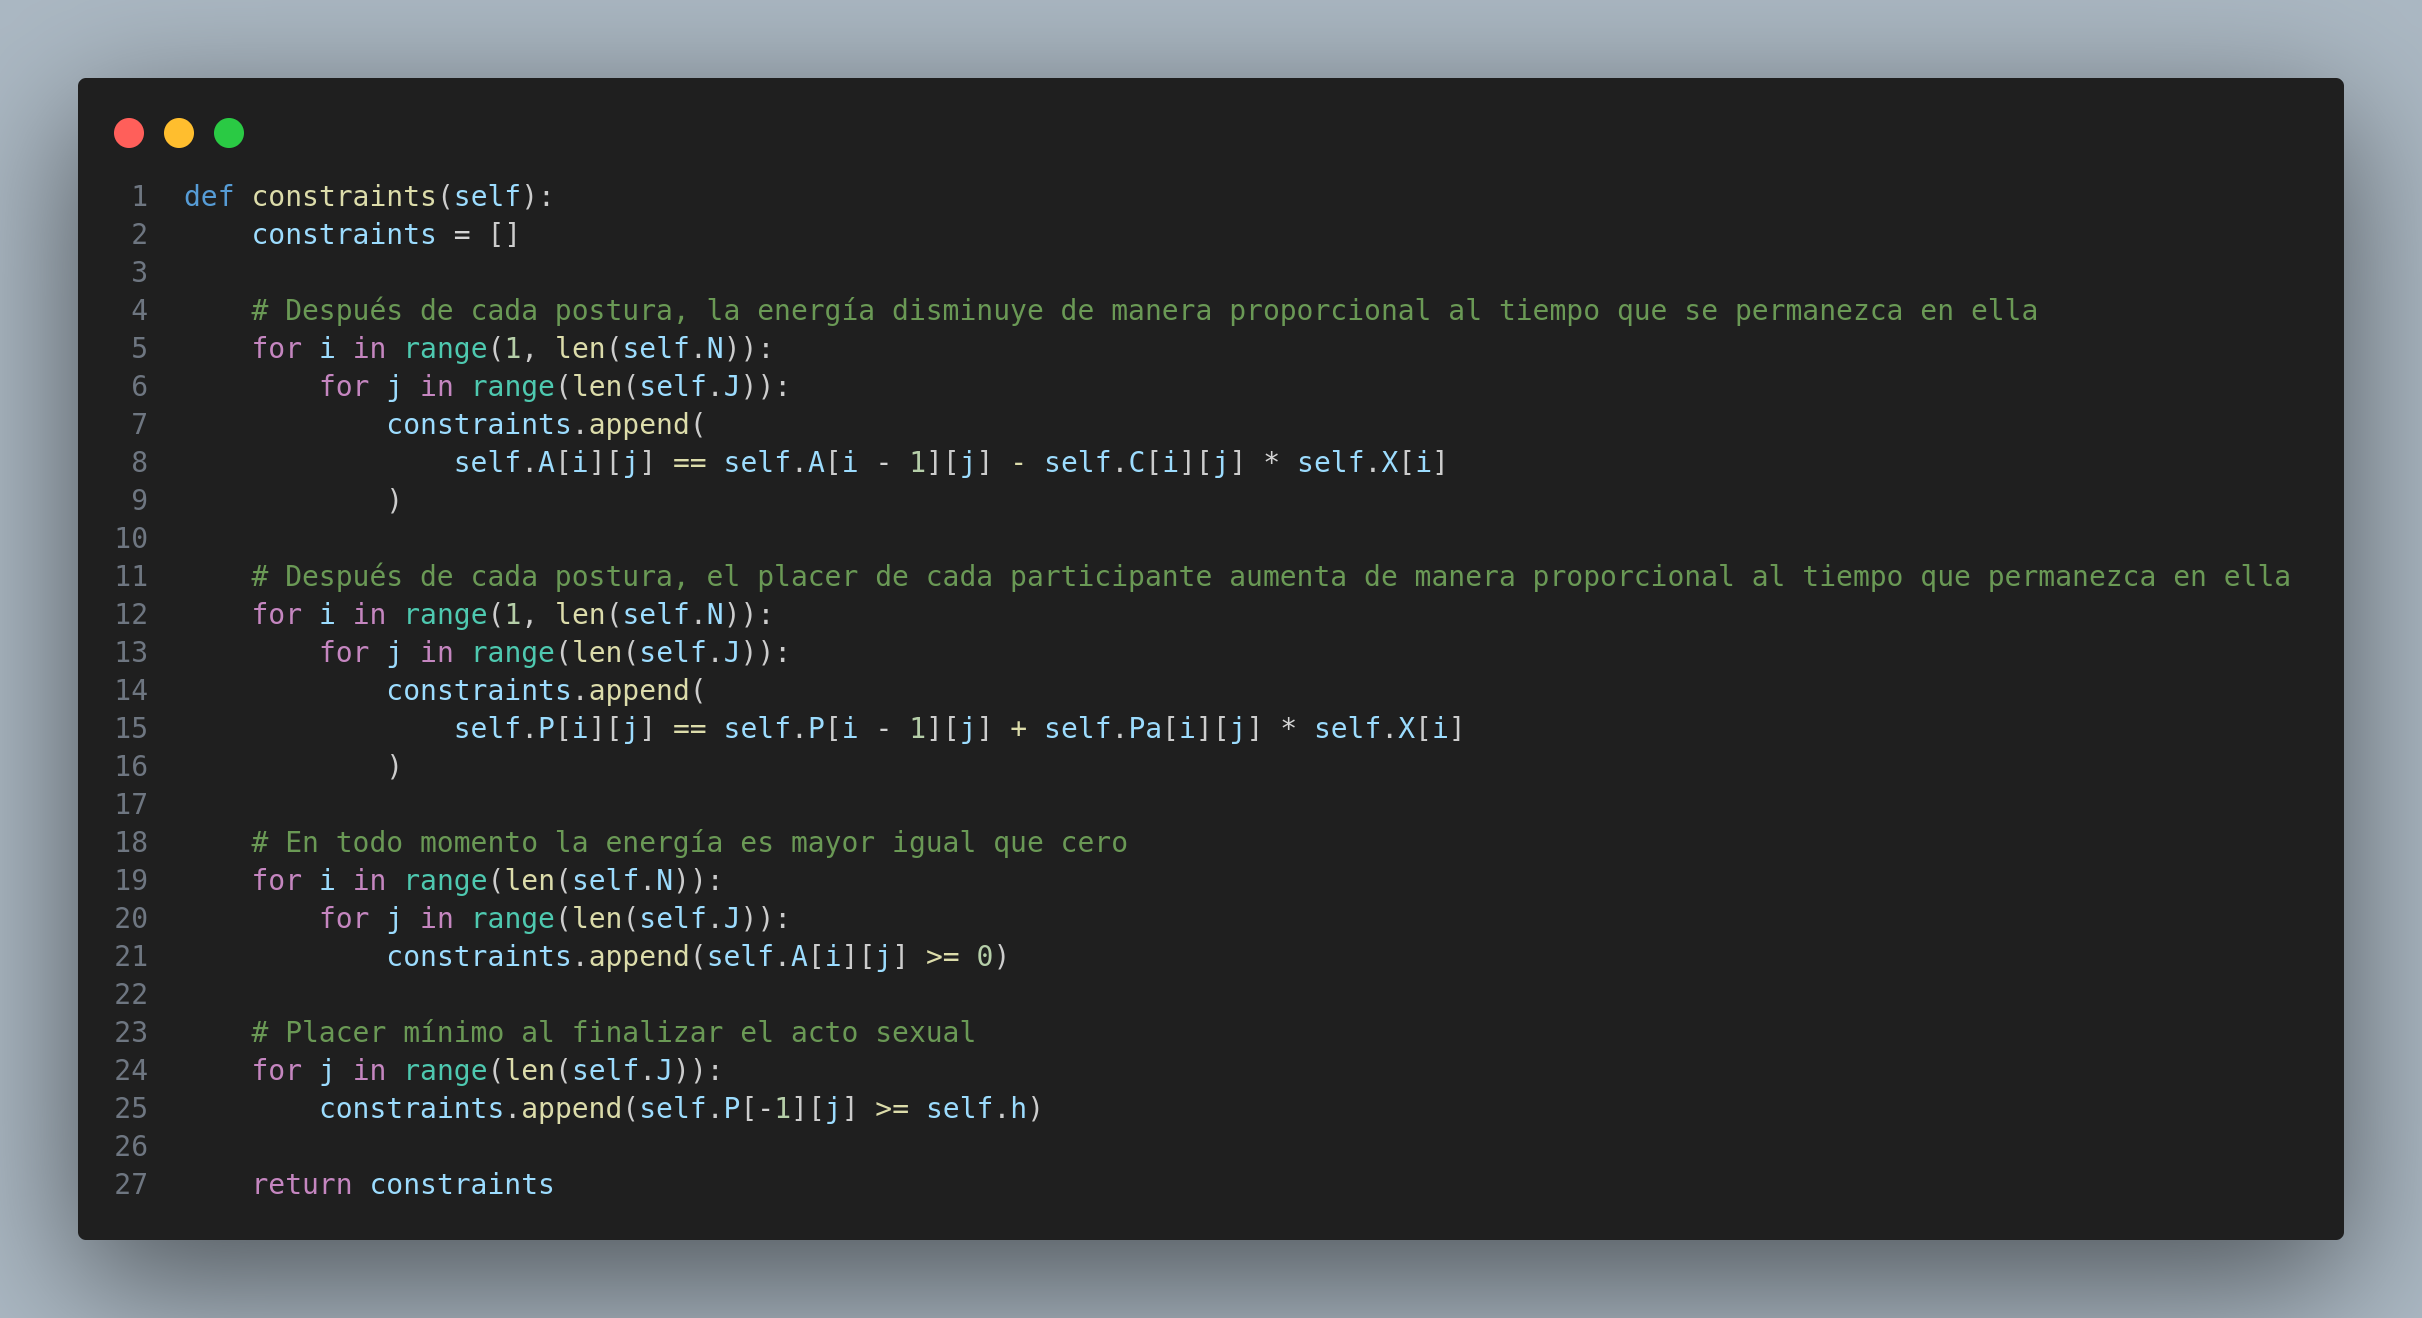
\includegraphics[width=0.7\textwidth]{images/max_min_constraints.png}
    \caption{Restricciones para el problema 2}
    \label{fig:rp2}
\end{figure}

\begin{figure}
    \centering
    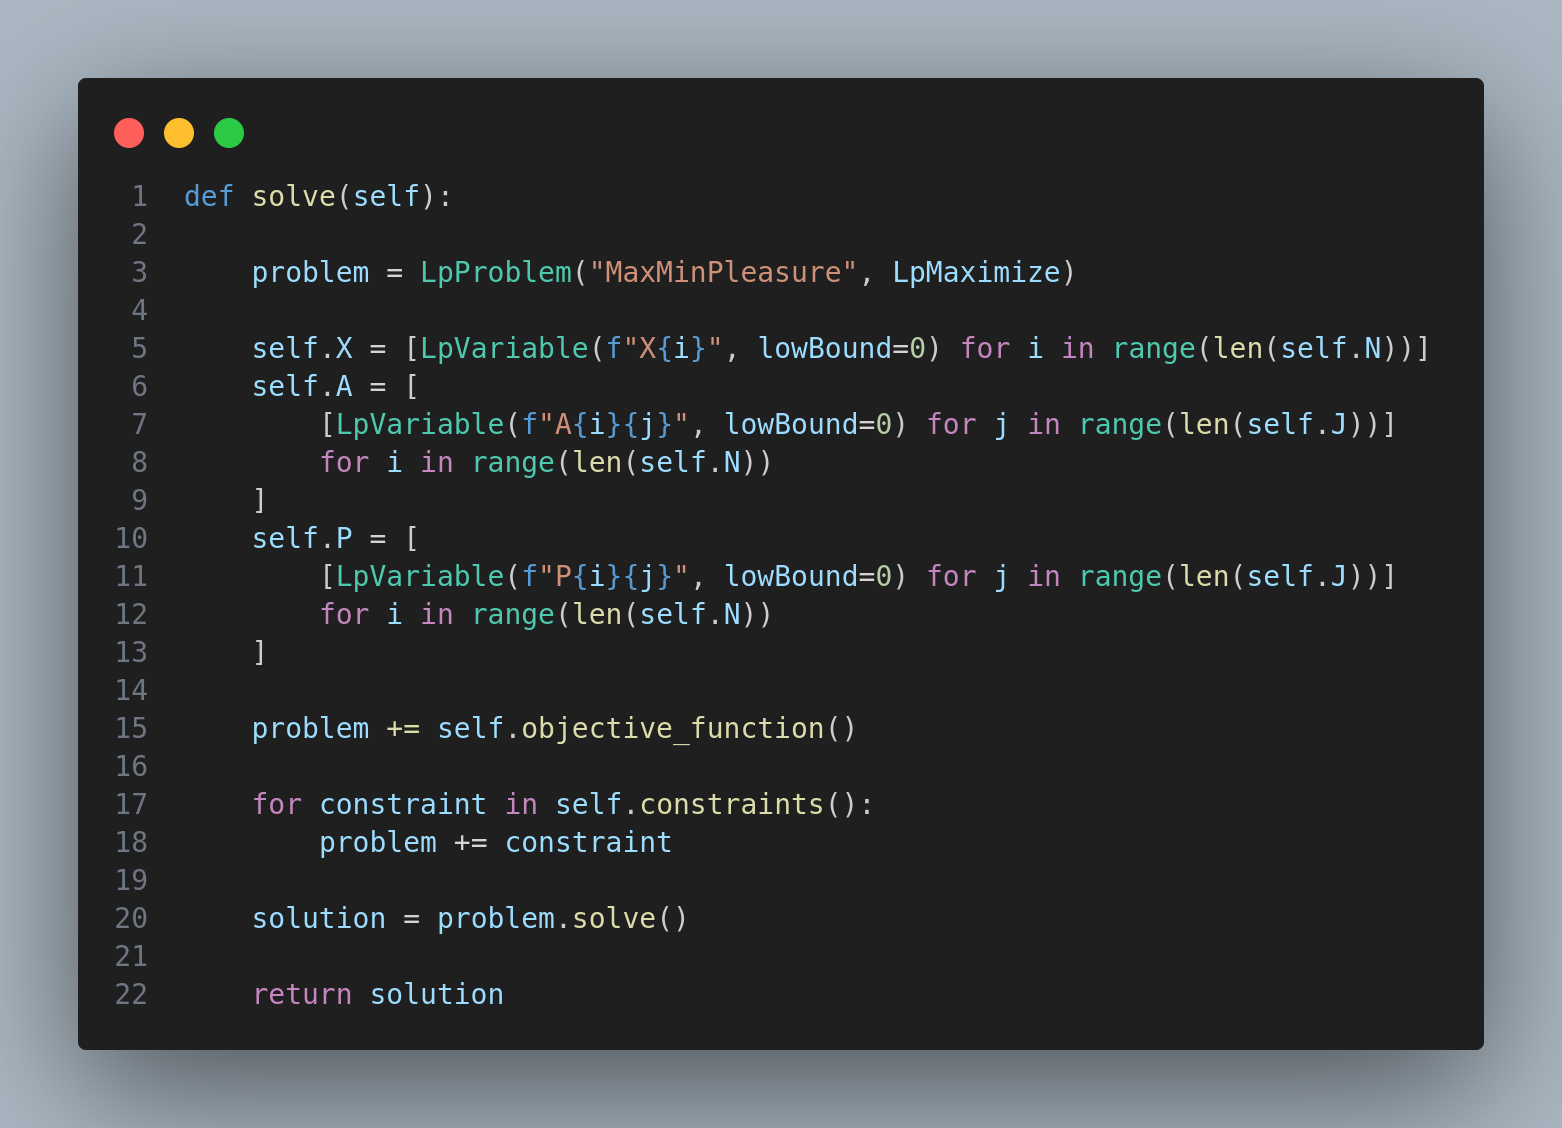
\includegraphics[width=0.7\textwidth]{images/max_min_solve.png}
    \caption{Resolución del problema 2}
    \label{fig:rs2} 
\end{figure}

\newpage

\section{Consideraciones}

Primeramente, abarcar todos los problemas planteados en la investigación no fue posible, por lo que se decidió implementar los problemas 1 y 2. La implementación de los problemas 3, 4 y 5 se deja como trabajo futuro.
\\
Los problemas pueden ser modelados teniendo en cuenta la preferencia sexual de cada participante, es decir, si el participante $J_i$ está dispuesto a ejecutar la postura dada con el participante $J_j$, con $0 \leq i <j \leq |J|$. 



\end{document}